\documentclass[11pt]{beamer}
\usepackage[T1]{fontenc}
\usepackage[utf8]{inputenc}
\usepackage[czech]{babel}
\usepackage{graphicx}
\usepackage{booktabs}
\usepackage{multirow}
\usepackage{amsmath}
\usepackage{array}
\usepackage{float}
\usepackage{adjustbox}
\usepackage{tikz}
\usetikzlibrary{positioning}

\usetheme{Madrid}
\usecolortheme{default}
\definecolor{farmdarkgreen}{HTML}{174C35}
\definecolor{farmgreenmid}{HTML}{245E43}
\definecolor{farmgreenlight}{HTML}{347253}
\definecolor{farmgreenpale}{HTML}{E7F0EA}
\setbeamercolor{structure}{fg=farmdarkgreen}
\setbeamercolor{palette primary}{bg=farmdarkgreen,fg=white}
\setbeamercolor{palette secondary}{bg=farmgreenmid,fg=white}
\setbeamercolor{palette tertiary}{bg=farmgreenlight,fg=white}
\setbeamercolor{palette quaternary}{bg=farmdarkgreen,fg=white}
\setbeamercolor{title}{fg=white,bg=farmdarkgreen}
\setbeamercolor{frametitle}{fg=white,bg=farmdarkgreen}
\setbeamercolor{block title}{fg=white,bg=farmdarkgreen}
\setbeamercolor{block body}{fg=black,bg=farmgreenpale}
\setbeamertemplate{navigation symbols}{}
\setbeamertemplate{caption}[numbered]
\setbeamerfont{title}{size=\Large}
\setbeamerfont{frametitle}{size=\large}

\title{Tým B: Osevní plán 2025}
\author{Návrh pro rozhodování}
\date{\today}

\begin{document}

\begin{frame}
  \titlepage
\end{frame}

\begin{frame}{Stručné představení problému}
  \vspace{0.3cm}
  \begin{center}
    \textbf{Jak rozdělit 1 000 ha mezi 20 plodin, když neznáme budoucí ceny, výnosy a riziko ztráty?}
  \end{center}
  \vspace{0.5cm}
  \begin{center}
    \begin{tikzpicture}
      \node[draw, rounded corners, fill=blue!10, minimum width=2.5cm] (A) {1 000 ha};
      \node[draw, rounded corners, fill=green!10, minimum width=2.5cm, right=1.6cm of A] (B) {20 plodin};
      \node[draw, rounded corners, fill=orange!20, minimum width=3.2cm, right=1.6cm of B] (C) {zisk + riziko};
      \draw[->, thick] (A) -- (B);
      \draw[->, thick] (B) -- (C);
    \end{tikzpicture}
  \end{center}
  \vspace{0.4cm}
  \begin{itemize}
    \item Rozhodování je pod silnou nejistotou.
    \item Cíl: maximalizovat zisk, ale ne přitom nechat otevřenou pravděpodobnost velké ztráty.
  \end{itemize}
\end{frame}

\begin{frame}{Vlastní formulace zadání a cílů projektu}
  \begin{block}{Zadání}
    Navrhnout osevní plán pro rok 2025, který respektuje nejistotu cen, výnosů a jejich vzájemné závislosti.
  \end{block}
  \vspace{0.3cm}
  \begin{block}{Cíle}
    \begin{itemize}
      \item vytvořit rozdělení ploch s vyšším očekávaným ziskem,
      \item současně zohlednit riziko nejhorších scénářů,
      \item porovnat varianty s různou averzí k riziku
    \end{itemize}
  \end{block}
\end{frame}

\begin{frame}{Jak se k výsledkům došlo}
  \begin{itemize}
    \item \textbf{Vstupní data:} roky 1993--2024 pro ceny a výnosy, náklady 2024 a inflaci CPI; všechny predikce se odhadují jen z dat známých ke konci roku 2024.
    \item \textbf{Výběr modelu:} pro ceny i výnosy se porovnávají více modelů a vybírá se ten s nejlepším out-of-sample výkonem podle CRPS a MAE.
    \item \textbf{Scénáře:} z historických chyb se generuje 5 000 společných scénářů pro ceny a výnosy; tím se zachovají závislosti mezi plodinami a neřeší se každá plodina izolovaně.
    \item \textbf{Optimalizace:} hledáme osevní plán maximálního zisku s penalizací nejhorších 10\% scénářů podle funkce \(\max_x (1-\lambda)E[Z(x)] + \lambda \mathrm{CVaR}_{10}[Z(x)]\).
  \end{itemize}
  \vspace{0.15cm}
  \begin{block}{Omezení úlohy}
    \begin{equation*}
      \sum_i x_i = 1000, \quad 0 \le x_i \le 250, \quad \sum_{i \in \text{zelenina}} x_i \le 200.
    \end{equation*}
  \end{block}
\end{frame}

\begin{frame}{Analýza a výsledky: hlavní výsledky}
  \begin{block}{Výkonnost a riziko}
    \begin{itemize}
      \item Ceny: zlepšení proti naivnímu modelu je malé, ale pozitivní.
      \item Výnosy: zlepšení je výraznější, což je klíčové pro plánování.
      \item U některých plodin je pravděpodobnost záporné marže vysoká i při přiměřeně dobrém očekávání.
    \end{itemize}
  \end{block}
  \vspace{0.1cm}
  \begin{center}
    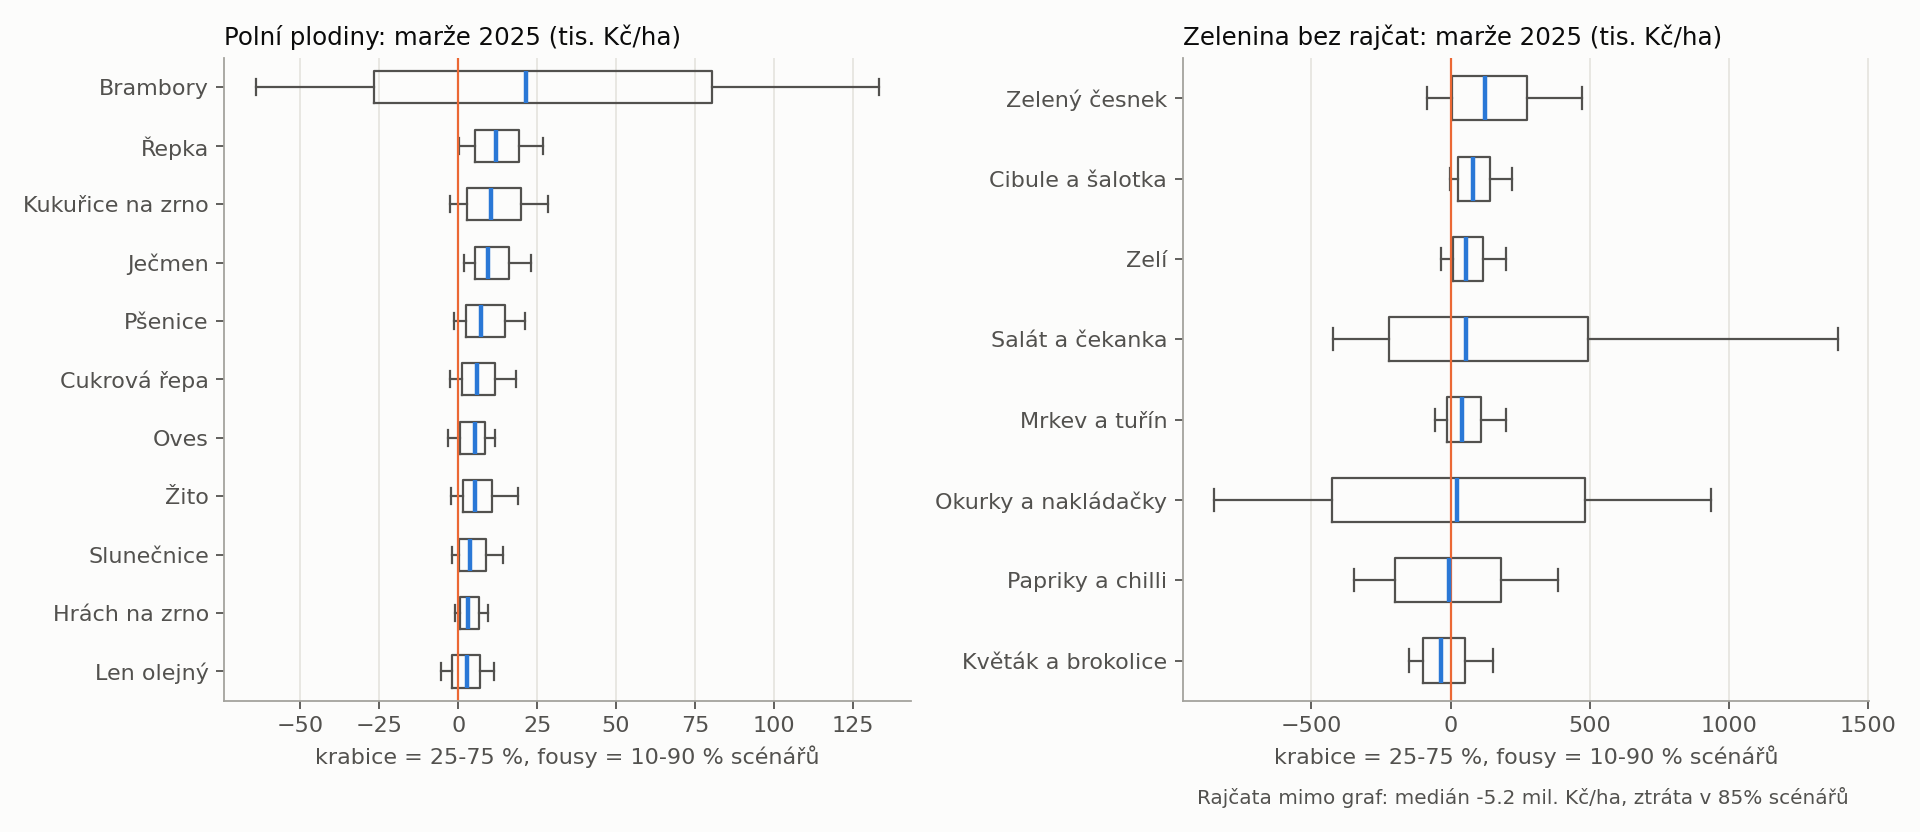
\includegraphics[width=0.78\textwidth]{vystupy/graf_marze_2025.png}
  \end{center}
\end{frame}

\begin{frame}{Citlivost na parametr \(\lambda\)}
  \begin{footnotesize}
  \begin{tabular}{lrrr}
    \toprule
    \(\lambda\) & Očekávaný zisk & CVaR10 & P(ztráta) \\
    \midrule
    0.0 & 86 920 496 & -100 950 489 & 33.5\% \\
    0.1 & 86 920 496 & -100 950 489 & 33.5\% \\
    0.25 & 76 141 359 & -51 843 029 & 23.9\% \\
    0.4 & 55 558 133 & -9 414 739 & 8.8\% \\
    0.5 & 50 342 532 & -2 936 384 & 5.7\% \\
    0.6 & 43 078 314 & 2 790 565 & 2.7\% \\
    0.75 & 36 035 577 & 6 486 591 & 0.8\% \\
    0.9 & 33 073 938 & 7 108 977 & 0.4\% \\
    1.0 & 31 635 786 & 7 189 994 & 0.4\% \\
    \bottomrule
  \end{tabular}
  \end{footnotesize}
  \vspace{0.25cm}
  \begin{block}{Interpretace}
    \begin{itemize}
        \item Zvyšování \(\lambda\) snižuje zisk, ale výrazně omezuje extrémní ztráty. 
        \item  Pro predikce jsme vybrali \(\lambda = 0.5\) jako referenční variantu, která nabízí vyvážený kompromis mezi očekávaným ziskem a rizikem.
    \end{itemize}
  \end{block}
\end{frame}

\begin{frame}{Vybrané plodiny pro \(\lambda=0.5\)}
  \begin{center}
     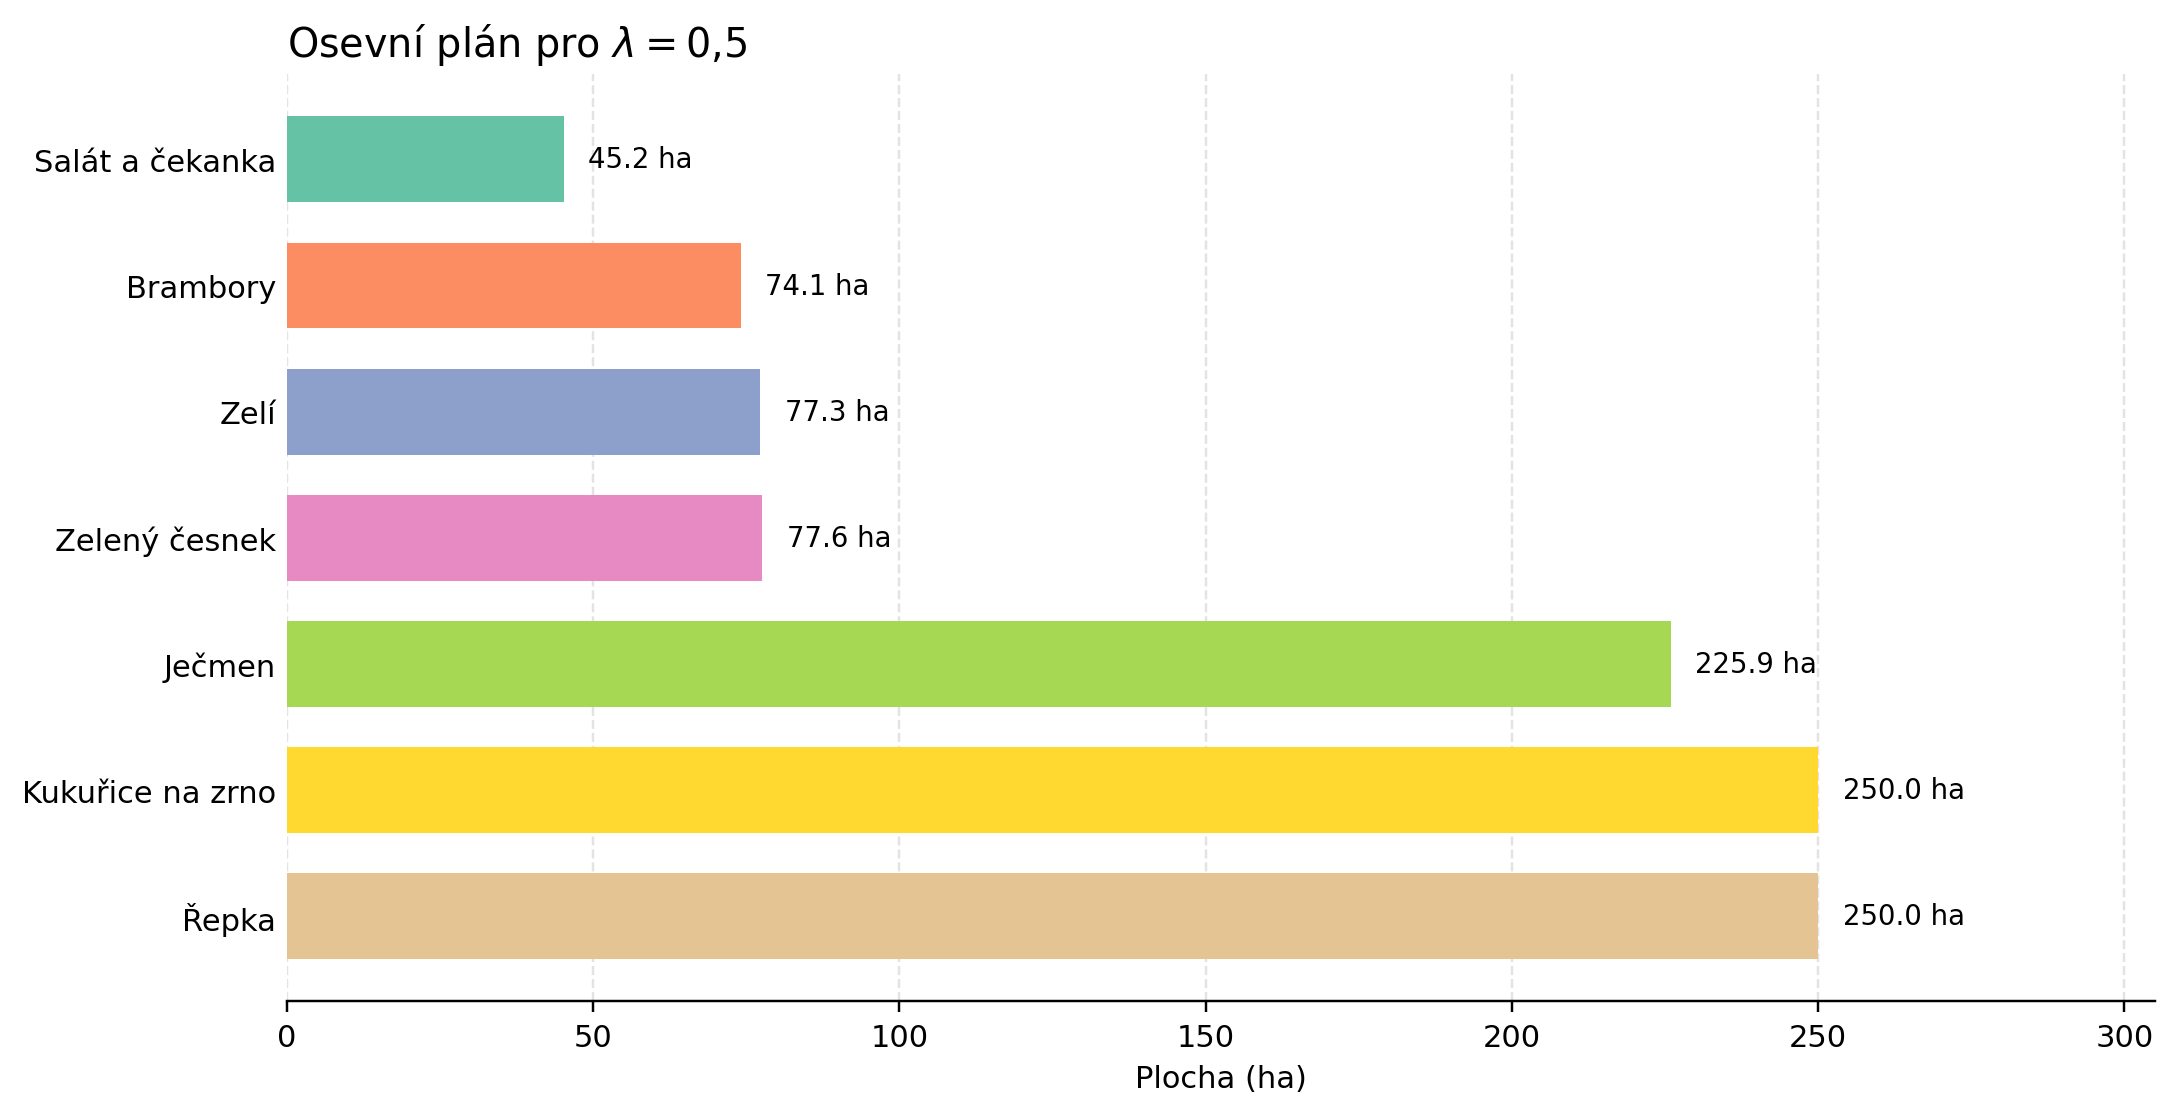
\includegraphics[width=1.0\textwidth]{vystupy/graf_plan_lambda_05_histogram.png}
  \end{center}
  \vspace{0.15cm}
  \begin{footnotesize}
    Celkem 1 000 ha je rozděleno především mezi kukuřici, řepku, ječmen a menší zálohy zelenin. Největší redukce oproti agresivnímu scénáři jde na brambory a salát, které jsou citlivější na výkyvy výnosu a ceny.
  \end{footnotesize}
\end{frame}

\begin{frame}{Doporučení a implikace}
  \begin{block}{Doporučení}
    \begin{itemize}
      \item Použít \(\lambda = 0.5\) jako referenční rozhodovací variantu.
      \item Pro konzervativnější vedení lze přejít k \(0.6\) až \(0.75\), pro agresivnější k \(0.25\) až \(0.4\).
      \item Před realizací nahradit národní údaje reálnými daty farmy.
    \end{itemize}
  \end{block}
\end{frame}

\begin{frame}{Limity analýzy}
  \begin{itemize}
    \item \textbf{Data:} národní roční výnosy místo farmových, krátký časový řetězec a omezený soubor extrémních událostí.
    \item \textbf{Metody:} predikce nemohou zohlednit všechny ekonomické a klimatické šoky; model odhaduje, ne vysvětluje všechny příčiny.
    \item \textbf{Provoz:} náklady, logistika, práce, investice a parcelní omezení nejsou plně modelované.
    \item \textbf{Udržitelnost:} model nehodnotí vodu, půdu, biodiverzitu, emise ani pracovní náročnost.
  \end{itemize}
\end{frame}

\begin{frame}{Diskuze nad rámec zadání}
  \begin{block}{Kritické zhodnocení}
    
    \begin{itemize}
      \item Národní data neprokázala statisticky významnou dvojici plodin, kterou by bylo rozumné zakázat.
      \item To neznamená, že na konkrétní farmě neexistuje silná lokální korelace.
    \end{itemize}
  \end{block}
\end{frame}

\end{document}
